% vi: tw=79
\documentclass[10pt, a4paper]{article}
\usepackage{lrec2016}
\usepackage{multibib}
\newcites{languageresource}{Language Resources}

\usepackage{amsmath}
\usepackage{booktabs}
\usepackage{multirow}
\usepackage{graphicx}
\usepackage{synttree}
\usepackage{times}
%\usepackage{url}
%\usepackage{hyperref}
\usepackage{latexsym}

\title{MyTitle}

\name{Adam Kovacs}
\address{MyAdress}

\abstract{
    MyAbstract
\newline 
\Keywords{semantics, lexicon, knowledge representation} }
\begin{document}
\maketitleabstract

\section{Introduction}

In this paper I present a way of matching \texttt{WikiData} relations with arguments of \texttt{4lang} definitions. The \texttt{dict\_to\_4lang} tool automatically builds graphs from longman dictionary definitions. The full pipeline is
available for download under an MIT license at \texttt{http://github.com/kornai/4lang}. \texttt{WikiData} is a publicly available knowledge base and we can make triplets out of it in the form of predicate(argument1, argument2). If we can make an assumption that these arguments corresponds to each other and a set of patterns can be applied to them, then we can  convert a large amount of information from WikiData to the 4lang format and combine the two knowledge.


\section{Combine WikiData and 4lang}
\label{sec:Combine WikiData and 4lang}
The 4lang pipeline maps the output of the Standford dependency parser to subgraphs representing the words of each definition.  For example \texttt{father} is defined in longman as 
\texttt{male parent}. 
The dictto4lang tool uses this definition to build a 4lang graph seen in Figure \ref{fig:father}. If we have a triplet coming from the WikiData knowledge base such as father(Az-Zahir Ghazi, Saladin) and we are ready to make an assumption that the second argument corresponds with the only IS A relation of out graph, then we can combine the fact with the longman definiton to obtain a new graph shown in Figure \ref{fig:fathernew}. We have a new machine a IS A relation, the \texttt{Saladin}~$\xrightarrow0$~\texttt{male} 0 edge that wasnt present before. We can see that we could obtain a completely new information which was unknown from the definition graph and from the Wikidata alone, and could only be present from the combination of the two.
If we want to build 4lang graphs automatically from WikiData, we will require a method for matching these relations, as in the case above. The result will have to be reviewed, and only the reasonable ones have to be selected. If we can apply patterns to these triplets and definitons, we can have a large amount of information retrieved from the combination of the two.


\begin{figure}
\centering
    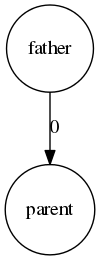
\includegraphics[scale=0.5]{father.png}
\caption{4lang definition of \texttt{father}.}
\label{fig:father}
\end{figure}

\begin{figure}
\centering
    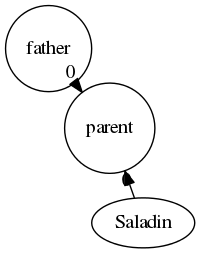
\includegraphics[scale=0.5]{fathernew.png}
\caption{4lang definition of \texttt{fathernew}.}
\label{fig:fathernew}
\end{figure}

\section{Methods}
\label{sec:Methods}
From the examination of the WikiData triplets, we can have a suspicion that if we say have a 0 edge in our definition graph \texttt{predicate}~$\xrightarrow0$~\texttt{X} then in our new graph coming from the combination of the WikiData and the 4lang graph, a machine looks like \texttt{arg2}~$\xrightarrow0$~\texttt{X} most likely going to have a place. And if we have an edge \texttt{predicate}~$\xrightarrow2$~\texttt{X} in our original graph, then we will have an  edge \texttt{arg1}~$\xrightarrow0$~\texttt{X} in the newly constructed graph. As we can see in Figure \ref{fig:creator} and \ref{fig:creatornew} new machines appeared such as \texttt{OpenCart}~$\xrightarrow0$~\texttt{thing} and \texttt{Daniel Kerr}~$\xrightarrow0$~\texttt{made} both of these appear to be valid information thanks to out pattern. Of course this is an ideal situation, this will not be always the case, there are many factors to be considered, when we apply these patterns to out data. We have to take into account the fact, that the triplets coming from the WikiData are not always going to be valid information. This case can be seen in Figure \ref{fig:tributary} and Figure \ref{fig:Tributarynew}, where one of the arguments of a WikiData triplet was \texttt{novalue}, so the edge created from the triplet does not holds any information. There are cases, when the originally created graph is not completely parsed right from the definition. \texttt{flag} is definition in longman is: \texttt {piece of cloth with a coloured pattern or picture on it that represents a country}. The definition graph built from this definition is in Figure \ref{fig:flag}. The machine \texttt{flag}~$\xrightarrow0$~\texttt{piece} obviously does not contain valid information, so the triplet flag(Belgium,flag of Belgium) with our current pattern would not add additional information to it. Our parser does not handle when there are multiple choices in a definition. For example longman defines employer \texttt{a person, company, or organization that employs people}. The graph constructed in Figure \ref{fig:employer} and \ref{fig:employernew}. We have an IS a edge \texttt{Central Intelligence Agency}~$\xrightarrow0$~\texttt{person} which we can presume is not a valid assumption, it would be rather a company. The next case, where out pattern can fail is when the WikiData and the longman has different definition of a word, it was the case when we examined the word Developer, which definition in longman was \texttt{a person or company that makes money by buying land and then building houses, factories etc on it} but the triplet in WikiData assumed it was a Software Developer as we can see Developer(De Blob, Blue Tongue Entertainment). s
 

\begin{figure}
\centering
    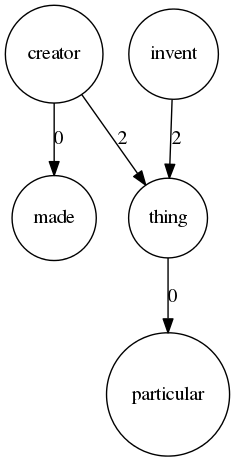
\includegraphics[scale=0.5]{creator.png}
\caption{4lang definition of \texttt{creator}.}
\label{fig:creator}
\end{figure}

\begin{figure}
\centering
    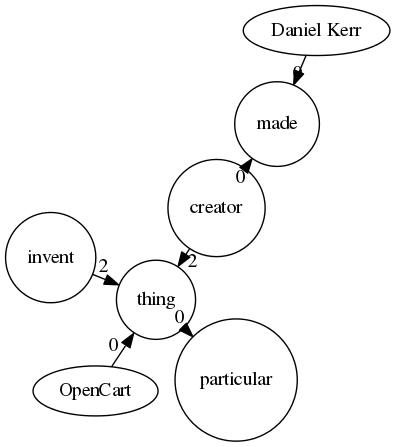
\includegraphics[scale=0.5]{creatornew.png}
\caption{4lang definition of \texttt{creatornew}.}
\label{fig:creatornew}
\end{figure}

\begin{figure}
\centering
    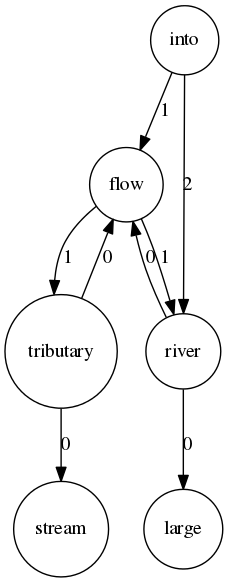
\includegraphics[scale=0.5]{tributary.png}
\caption{4lang definition of \texttt{tributary}.}
\label{fig:tributary}
\end{figure}

\begin{figure}
\centering
    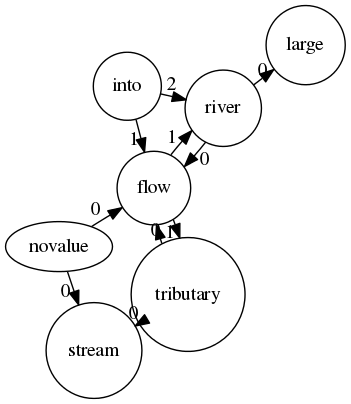
\includegraphics[scale=0.5]{tributarynew.png}
\caption{4lang definition of \texttt{tributarynew}.}
\label{fig:tributarynew}
\end{figure}

\begin{figure}
\centering
    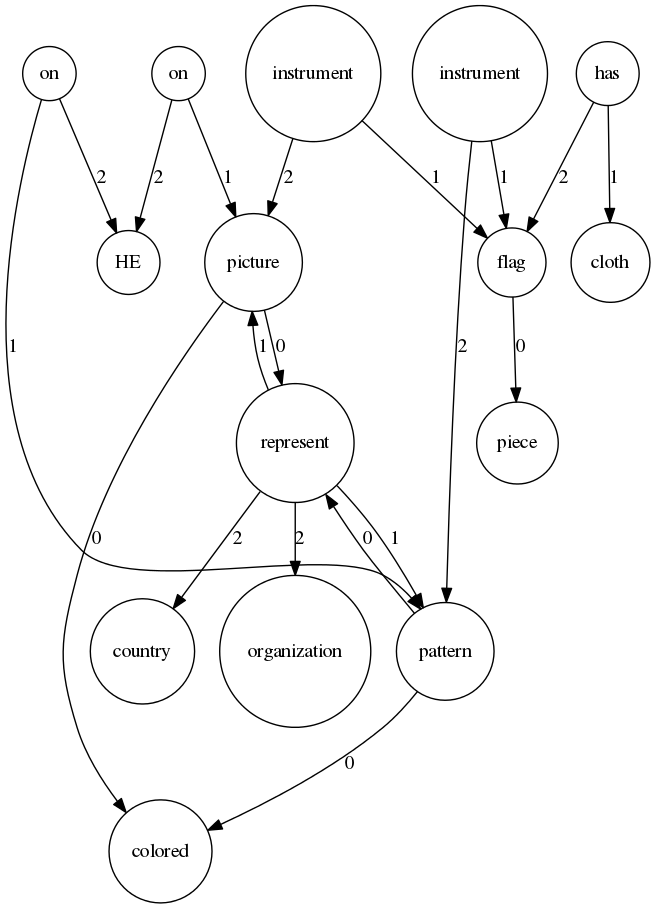
\includegraphics[scale=0.5]{flag.png}
\caption{4lang definition of \texttt{flag}.}
\label{fig:flag}
\end{figure}

\begin{figure}
\centering
    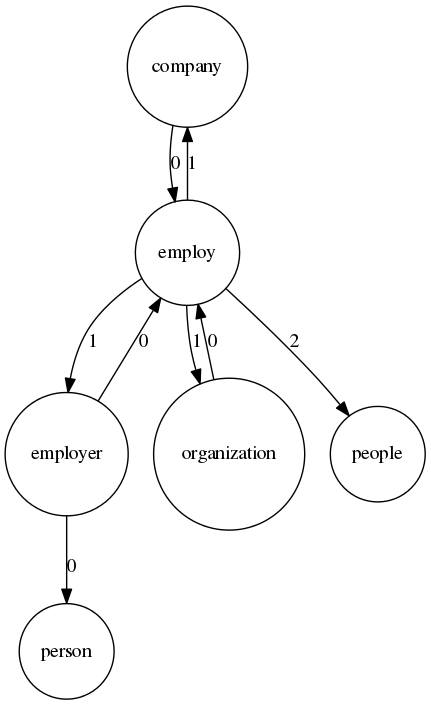
\includegraphics[scale=0.5]{employer.png}
\caption{4lang definition of \texttt{employer}.}
\label{fig:employer}
\end{figure}

\begin{figure}
\centering
    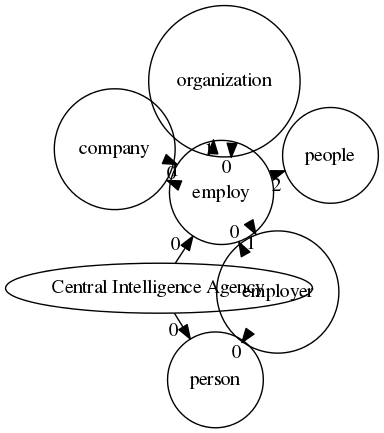
\includegraphics[scale=0.5]{employernew.png}
\caption{4lang definition of \texttt{employernew}.}
\label{fig:employernew}
\end{figure}

\section{The \texttt{4lang} formalism}
\label{sec:4lang}


\section{Building definition graphs}
\label{sec:defgraphs}



\section{Issues}
\label{sec:issues}


%nsd


\section{Evaluation}
\label{sec:eval}



\section{Expansion}
\label{sec:expansion}


\section{Applications}
\label{sec:applications}


 \section{Acknowledgements}
 The author wishes to thank Andr\'as Kornai, M\'arton Makrai, D\'avid Nemeskey,
 and two anonymous reviewers for their many useful comments on earlier versions
 of this paper.

\section{Bibliographical References}
\label{main:ref}

\bibliographystyle{lrec2016}
\bibliography{ml}


\end{document}
